\documentclass[8pt]{article}


\usepackage{arxiv}
\usepackage{titlesec}
\usepackage[utf8]{inputenc} % allow utf-8 input
\usepackage[T1]{fontenc}    % use 8-bit T1 fonts
\usepackage{hyperref}       % hyperlinks
\usepackage{url}            % simple URL typesetting
\usepackage{booktabs}       % professional-quality tables
\usepackage{amsfonts}       % blackboard math symbols
\usepackage{nicefrac}       % compact symbols for 1/2, etc.
\usepackage{microtype}      % microtypography
\usepackage{lipsum}
\usepackage{listings}
\usepackage{graphicx}
\usepackage{float}
\usepackage{multirow}
\usepackage{caption}
\usepackage{subcaption}
\usepackage{mathtools}
\usepackage[usenames,dvipsnames]{color}



\captionsetup{belowskip=0pt}

% Python style for highlighting
\newcommand\pythonstyle{\lstset{
language=Python,
basicstyle=\ttm,
morekeywords={self},              % Add keywords here
keywordstyle=\ttb\color{deepblue},
emph={MyClass,__init__},          % Custom highlighting
emphstyle=\ttb\color{deepred},    % Custom highlighting style
stringstyle=\color{deepgreen},
frame=tb,                         % Any extra options here
showstringspaces=false
}}


% Python environment
\lstnewenvironment{python}[1][]
{
\pythonstyle
\lstset{#1}
}
{}

\title{Predicting International Football Match Results}


\author{
 Group Name: \texttt{Group K}\\
  Department of Biomechanical Engineering\\
  University College London\\
  London, WC1E 6BT\\
}

\begin{document}
\maketitle

%\begin{abstract}

%\end{abstract}

%\small
\section{Introduction}
Having received a dataset of more than five thousand international football games that have taken place in the past 2 decades, the purpose of this work is to predict future international match results through machine learning and predictive modelling - employing numerous data processing and reconstruction techniques along the way. The dataset contains relevant information about the participants and the location of each game played, along with numerical evaluations of both teams. These evaluations include values such as the offence score of a team in a particular game, or the performance of their goalkeeper.

It must also be noted that the dataset is incomplete - with some match records sporadically missing values, and more seriously, some teams missing data points entirely. Hence, in order to improve the accuracy of the tested models and predictors, various methods of data pre-processing and reconstruction are employed. 

This report outlines the findings of the data exploration, the reconstruction of the missing values deemed critical to our model training, and the outcomes of several machine learning approaches; Support Vector Machine, Logistic Regression, k-Nearest Neighbours and Multiplayer Perceptron.

\section{Data Transformation and Exploration}
\label{sec:explorationw}
\subsection{Data Exploration}
The objective of the project is to develop a predictive model for the outcomes of football matches. After a thorough examination of the available data, it was determined that there is a strong correlation between the relative strength of the teams involved and the resulting outcome of the match. Accordingly, this correlation will be taken into account as a key factor in the development of the predictive model. 
Therefore, we mainly focus on the team position score features.

In order to gain a more comprehensive understanding of the position scores, a graph was plotted to illustrate the relationship between the position scores and FIFA rank (Figure 1). This representation allowed for a more lucid analysis of the data, and facilitated a deeper understanding of the underlying trends and patterns.

Upon inspection of the provided \textit{match\_history.csv} file, it became clear that numerous data points are missing. Throughout the dataset, for at least one country each, there is data missing from the \textit{offense\_score, midfield\_score, defense\_score} and \textit{goalkeeper\_score} fields. When reading the data, these missing values are interpreted as `NaN' - a value that cannot be used in any regression technique. Since the quality of a model's output is directly correlated to its input, as mentioned above, we tried numerous methods of handling the fact that these values are missing; in order to be able to train regression models properly with a complete dataset.
\begin{figure}[H]
    \centering
    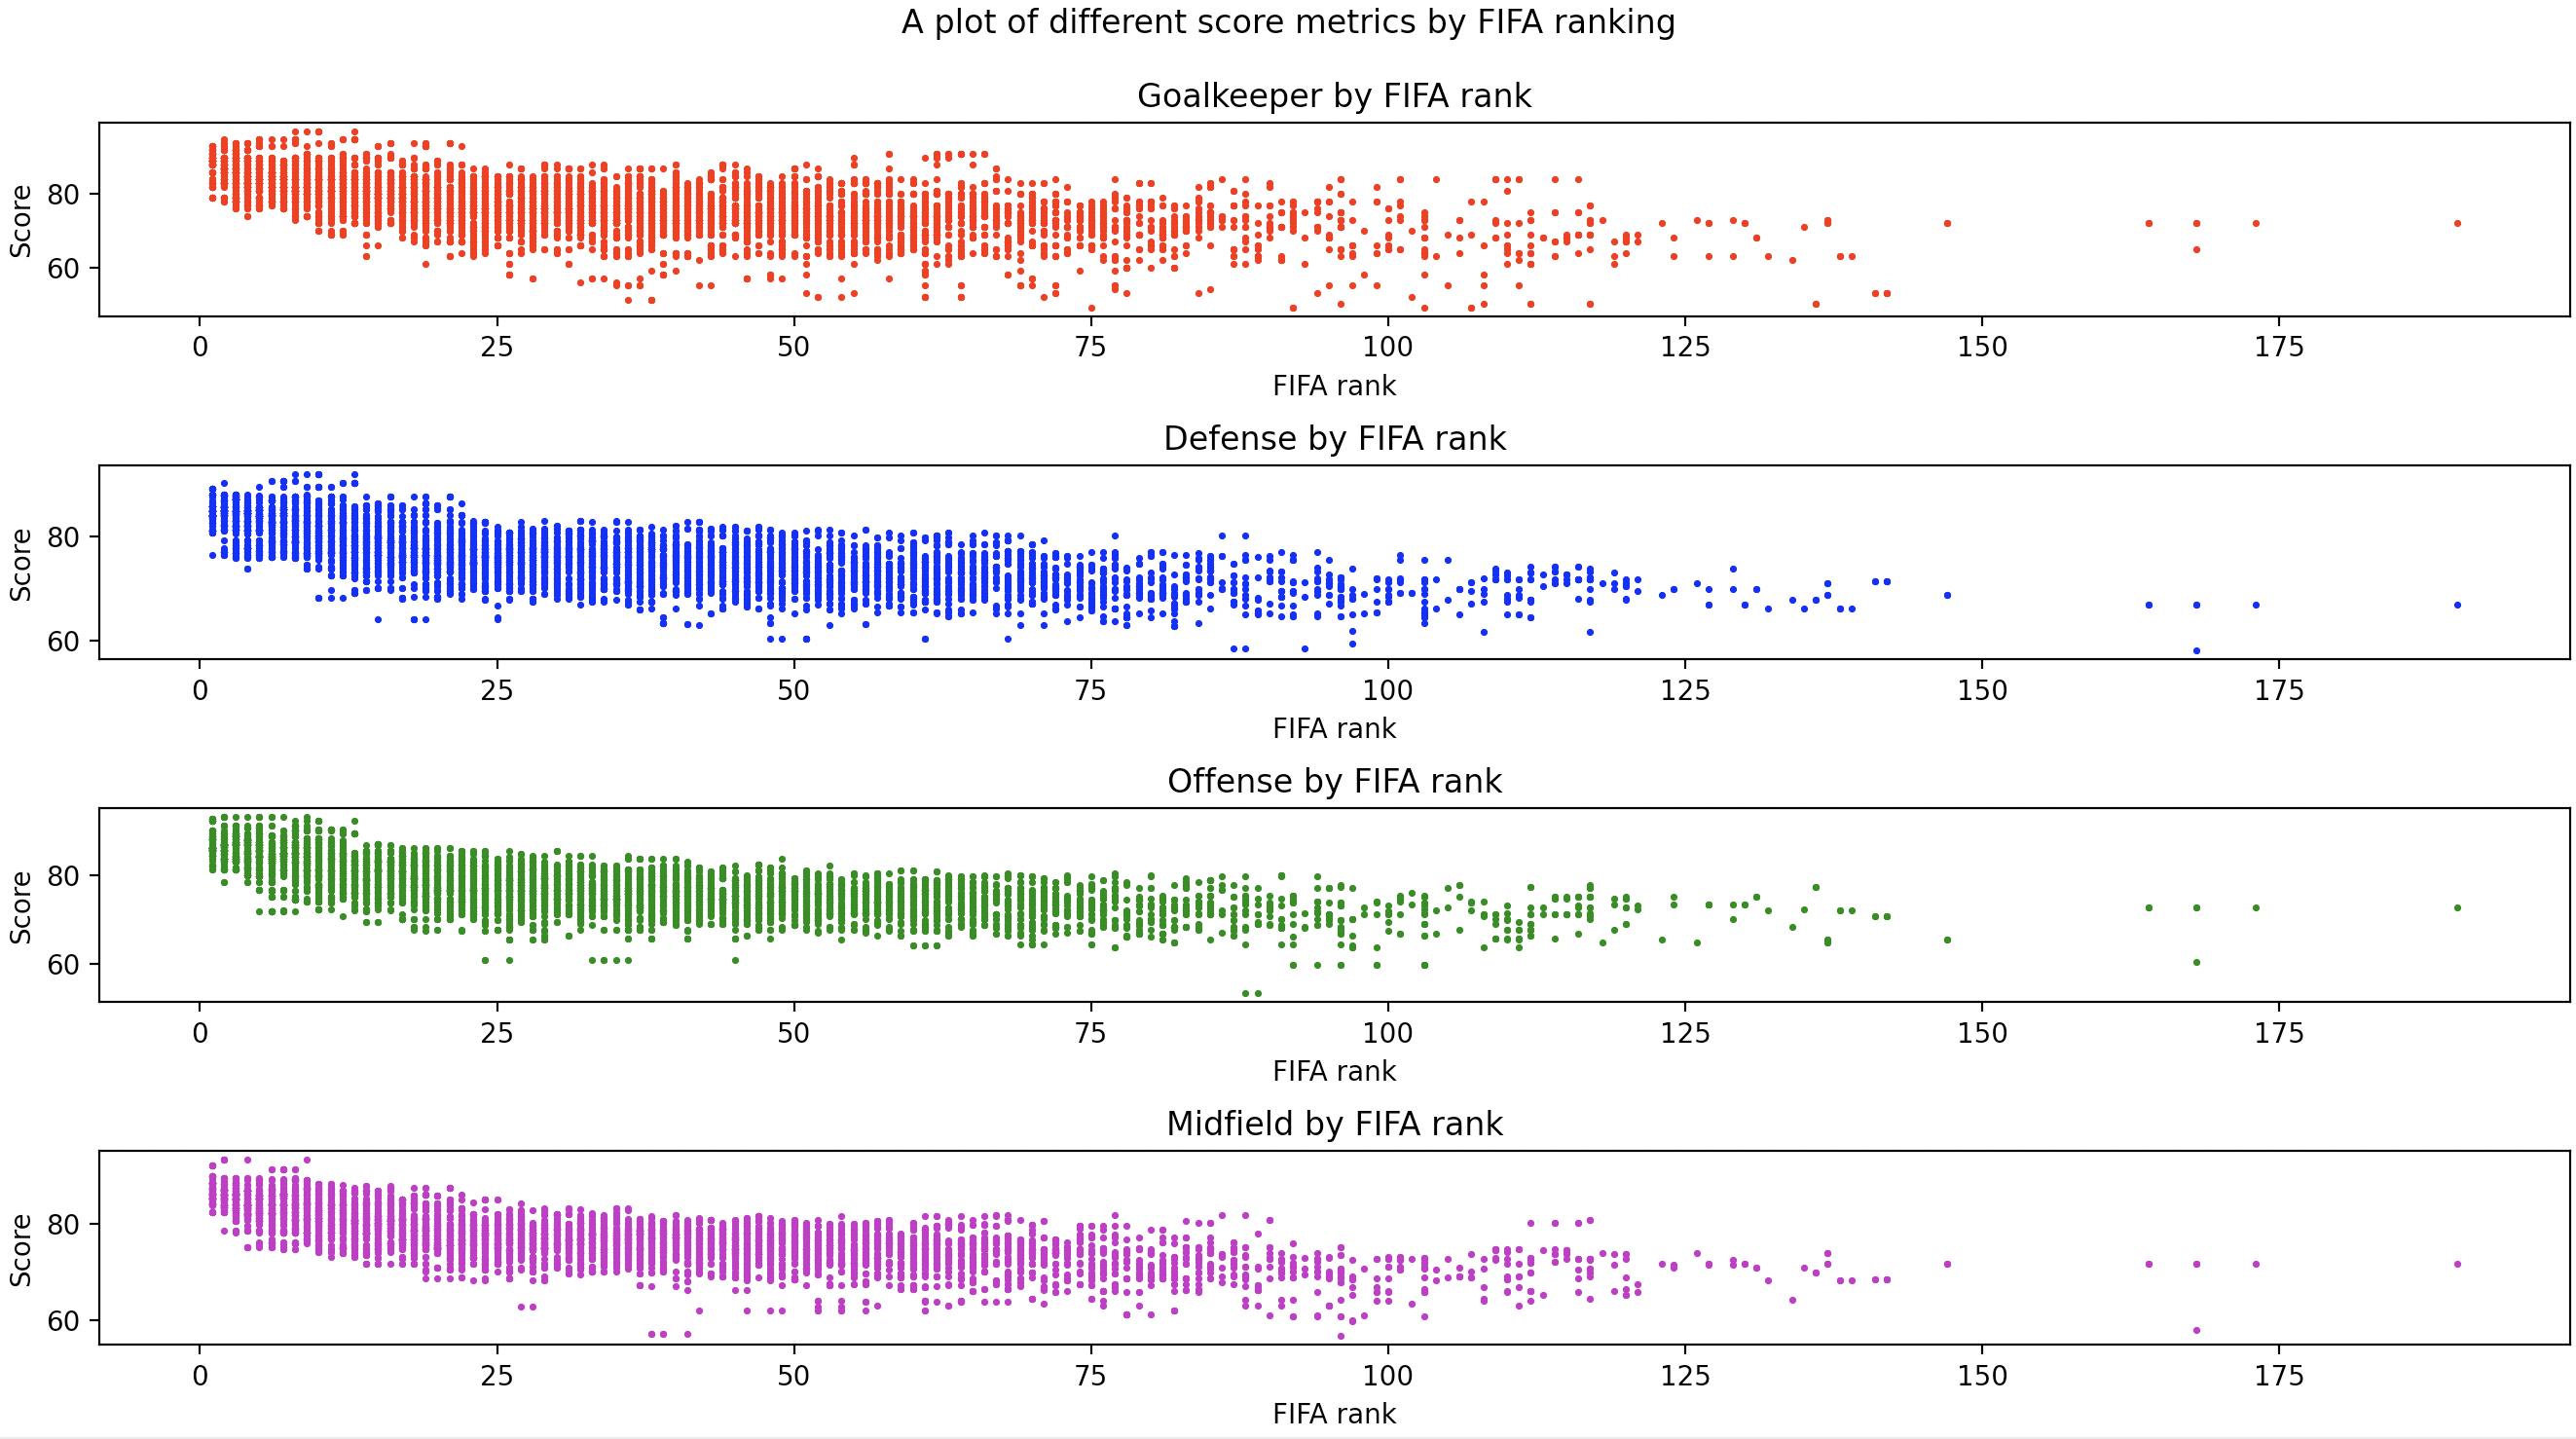
\includegraphics[scale=.3]{scores_plots.png}
    \caption{\textit{goalkeeper\_score, defense\_score, offense\_score, midfield\_score} plotted by country against said country's FIFA ranking.}
    \label{fig:scoreplots}
\end{figure}
\subsubsection{Types of Missing Data}
As previously stated, the efficacy of a model and the quality of the dataset are directly correlated - insufficient or poor quality data produces inaccurate and meaningless predictions. 
In our dataset, missing data can be categorised into two distinct types \cite{missing_data}: 
    1. Missing data which has some existing position values to predict them, we will call this TYPE1 missings
    2. Missing data which has no existing position values to predict them, we will call this TYPE2 missings
    
\begin{figure}[H]
    \centering
    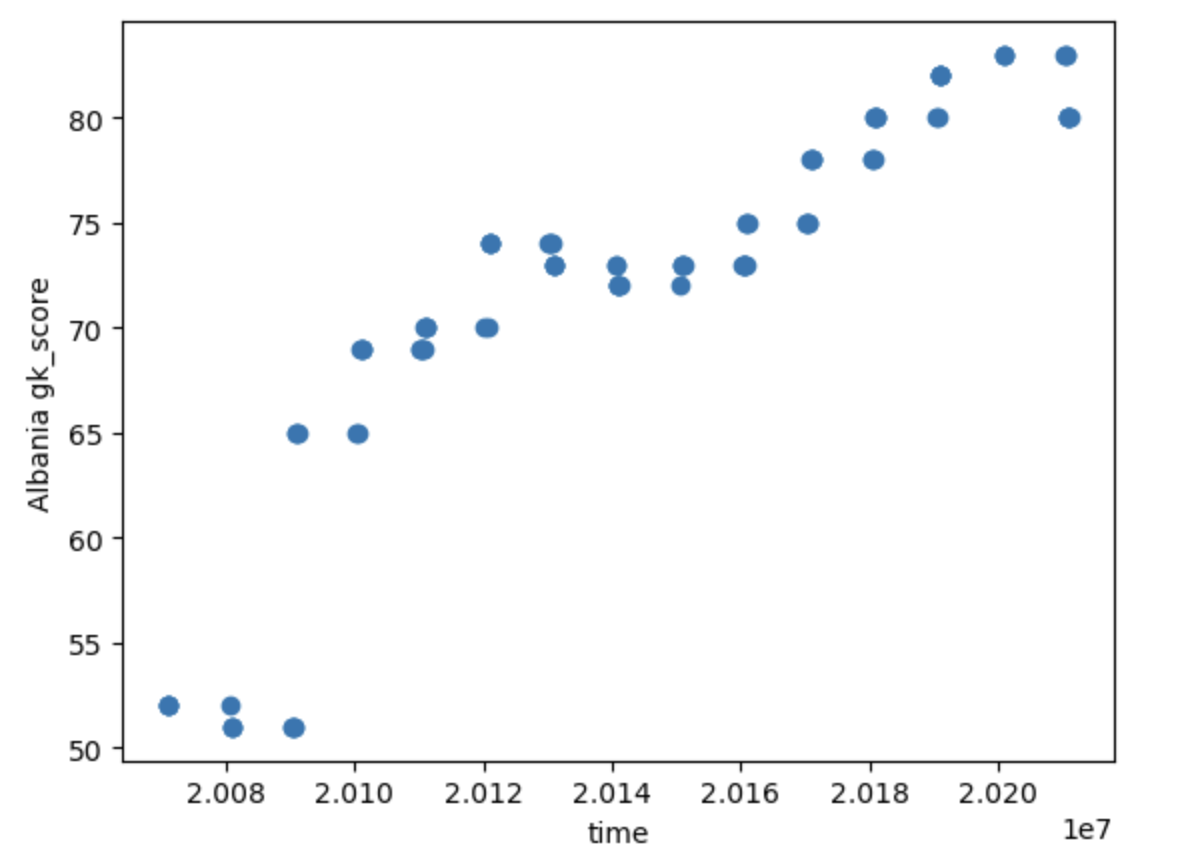
\includegraphics[scale=.3]{alb_gk_values.png}
    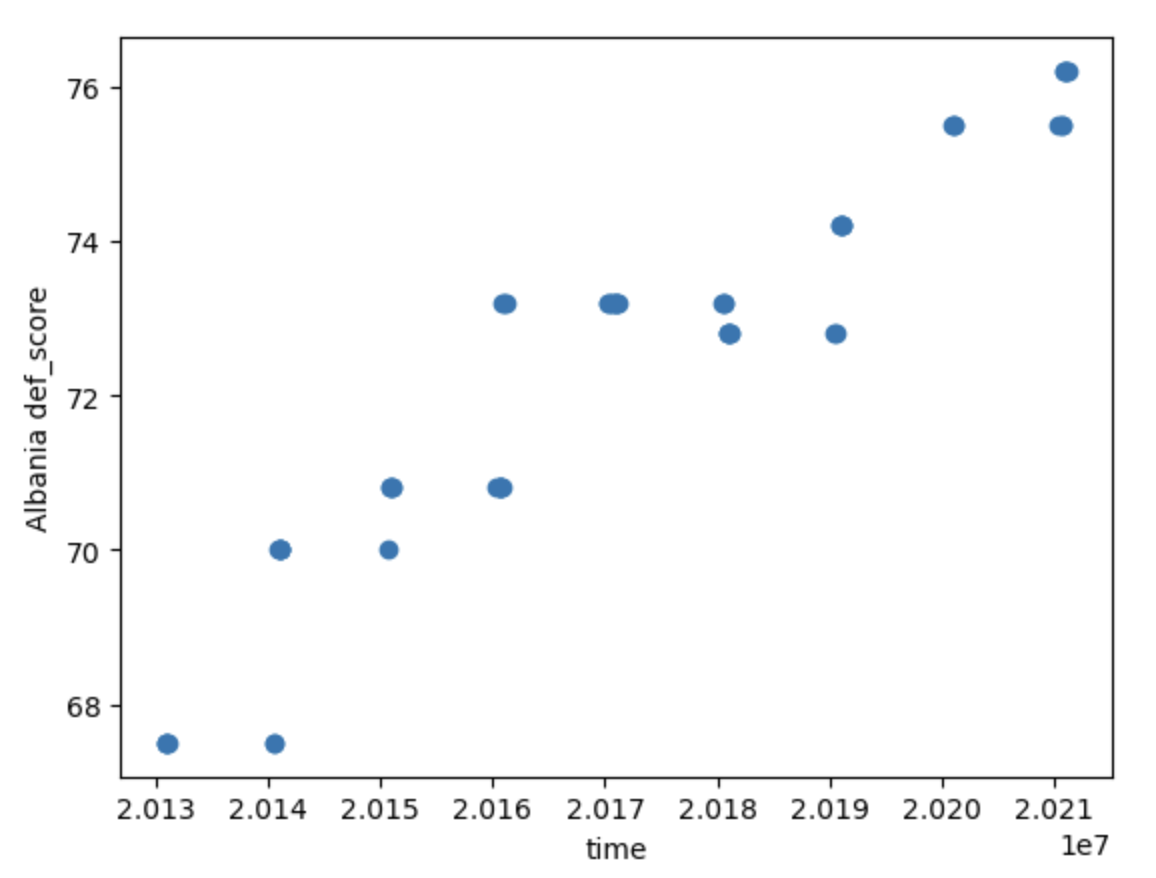
\includegraphics[scale=.3]{alb_def_values.png}
    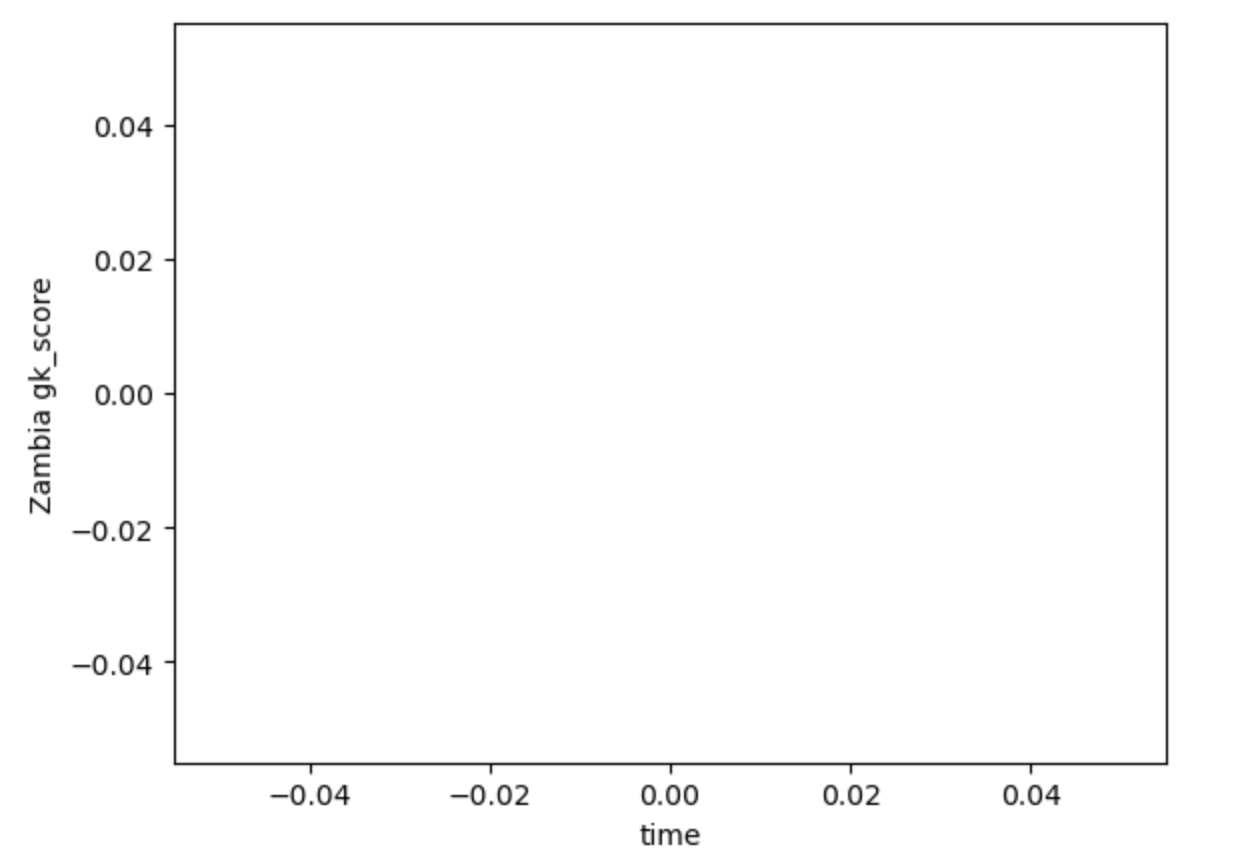
\includegraphics[scale=.3]{zam_gk_values.png}
    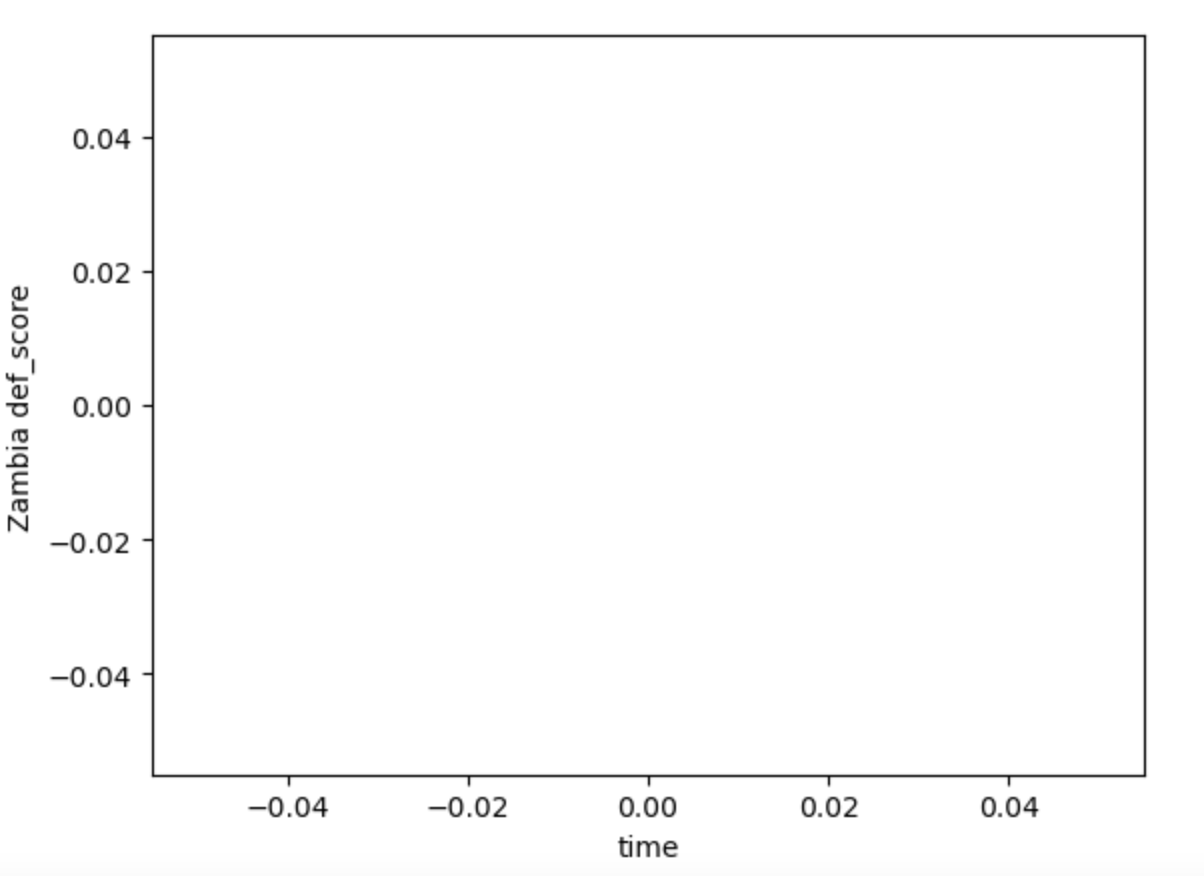
\includegraphics[scale=.3]{zam_def_values.png}
    \caption{plot of gk\_scores and def\_scores of Albania and Zambia, inside the dataset}
    \label{fig:posscores}
\end{figure}


From Figure 2, for example, Albania has some missing values for \textit{goalkeeper\_score} and \textit{defense\_score} however, inside the dataset exist values which may be examined to predict its missing values. In contrast, Zambia has no \textit{goalkeeper\_score} and \textit{defense\_score} throughout the entire dataset which adds a further layer of complexity.

\label{sec:exploration}
\subsection{Data Transformation}
\label{sec:miss sec}
\subsubsection{General Data Transformation}
Initially, to ease the process of constructing a prediction model, we transformed match\_result data [Win,Lose,Draw] into [1,0,-1].

\subsubsection{Simple Prediction of Missing Values}

\textbf{Replacing With Constant}\vspace{0.05cm}

Our initial approach was simply to find all `NaN' values after the dataset had been read and replace them with a zero. This is extremely fast to execute, however, leads to poor model performance since in most cases, zero is an inaccurate value to replace missing values - with almost all score features being valued above 50. This is evident when graphing the four aforementioned features - no country has a value for any of the aforementioned features that are remotely close to zero.

From Figure 1, since the values we were concerned with filling were all position scores, we decided to look at the distribution of these features to get a better understanding of what static values we could reasonably replace them with.

\begin{figure}[H]
    \centering
    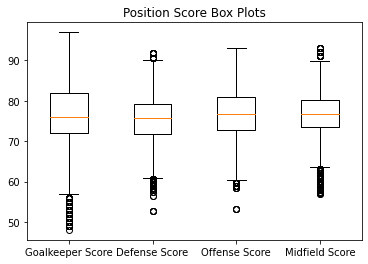
\includegraphics[scale=.6]{box_plots.png}
    \caption{Box plots for \textit{goalkeeper\_score, defense\_score, offense\_score,} and \textit{midfield\_score}.}
    \label{fig:boxplots}
\end{figure}
As shown in the \hyperref[fig:boxplots]{Figure 3}, all of the position features are roughly centred around 75, with tight inter-quartile ranges of about 10. Given that the whiskers didn't extend beyond 15 points above or below the median, this gave us confidence that taking a static value of 75 was reasonable in cases where data was missing. This method was simple and maintained efficiency at run time, while not skewing the data or providing any significant advantage to either team involved.

\textbf{Ignoring the Records}\vspace{0.05cm}

The most naïve approach to dealing with missing data in a dataset is to simply ignore the records that have missing values when training a model. This method is quick and simple to implement. Furthermore, this method's naïvety does not necessarily equate to poor performance. Overall, in the provided dataset of 5642 records, 1525 of them are missing at least one value, meaning that simply removing these rows to generate a new complete dataset, leaves 4117 records to use in model training. We found this to be more than enough to still achieve reasonable model accuracy for each method regression used.

\subsubsection{Advanced Prediction of Missing Values}
Since simply removing rows would be considered naive, we also approached predicting the missing values.

In order to predict the TYPE1 missings, we attempted to further explore the plotting of each position value sets according to the country. However, upon examination, it was observed that the overall tendency of the 151 plots of position value sets displayed a significant degree of variation.

As a result of a comprehensive analysis, it was determined that the undertaking of calculating each individual value would prove to be excessively time-consuming and labour-intensive. Despite the absence of a clear general tendency in the plotted graphs, an examination revealed that the range of scores was limited. As such, it was decided to utilize a more efficient method of determining the relevant metric, by calculating the average of the values and utilizing that as a replacement for the range of the values.
\begin{figure}[H]
    \centering
    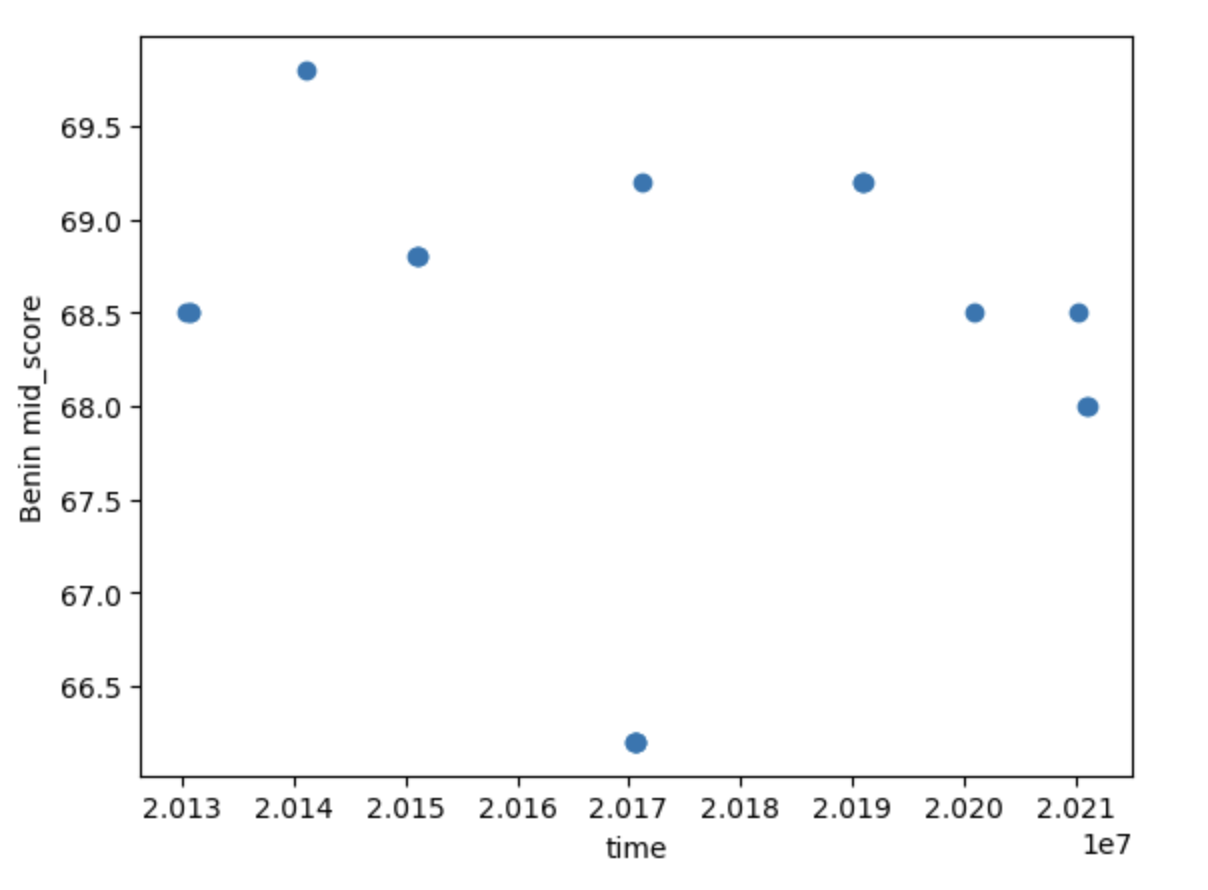
\includegraphics[scale=.3]{ben_mid_values.png}
    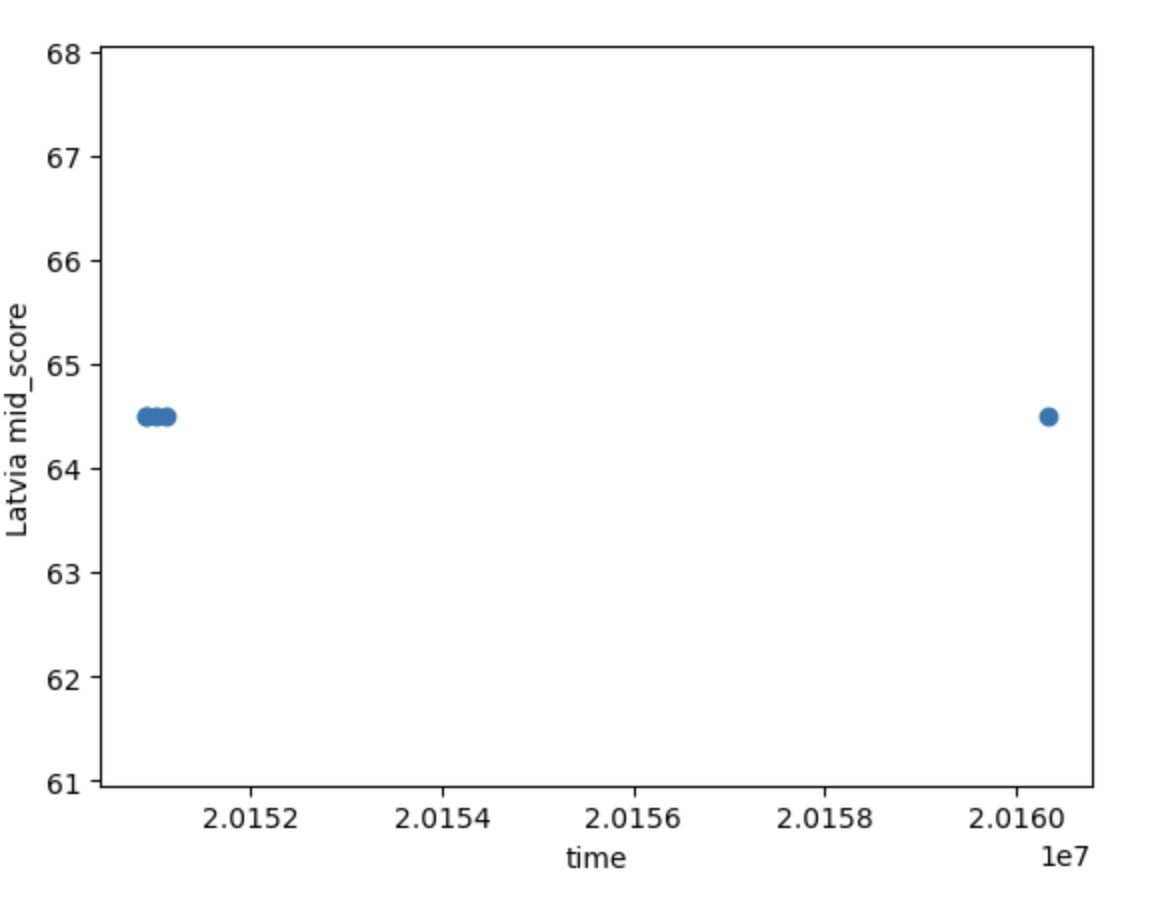
\includegraphics[scale=.3]{lat_mid_values.png}
    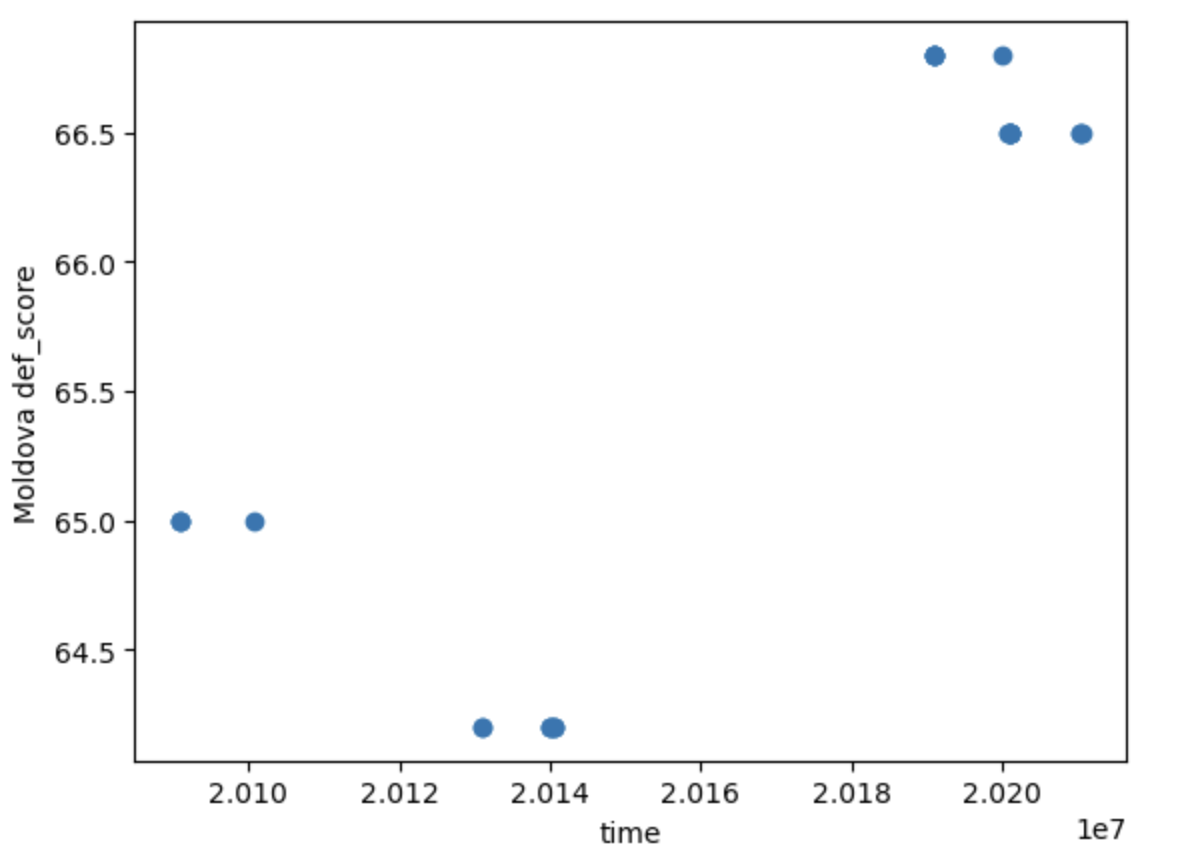
\includegraphics[scale=.3]{mol_def_values.png}
    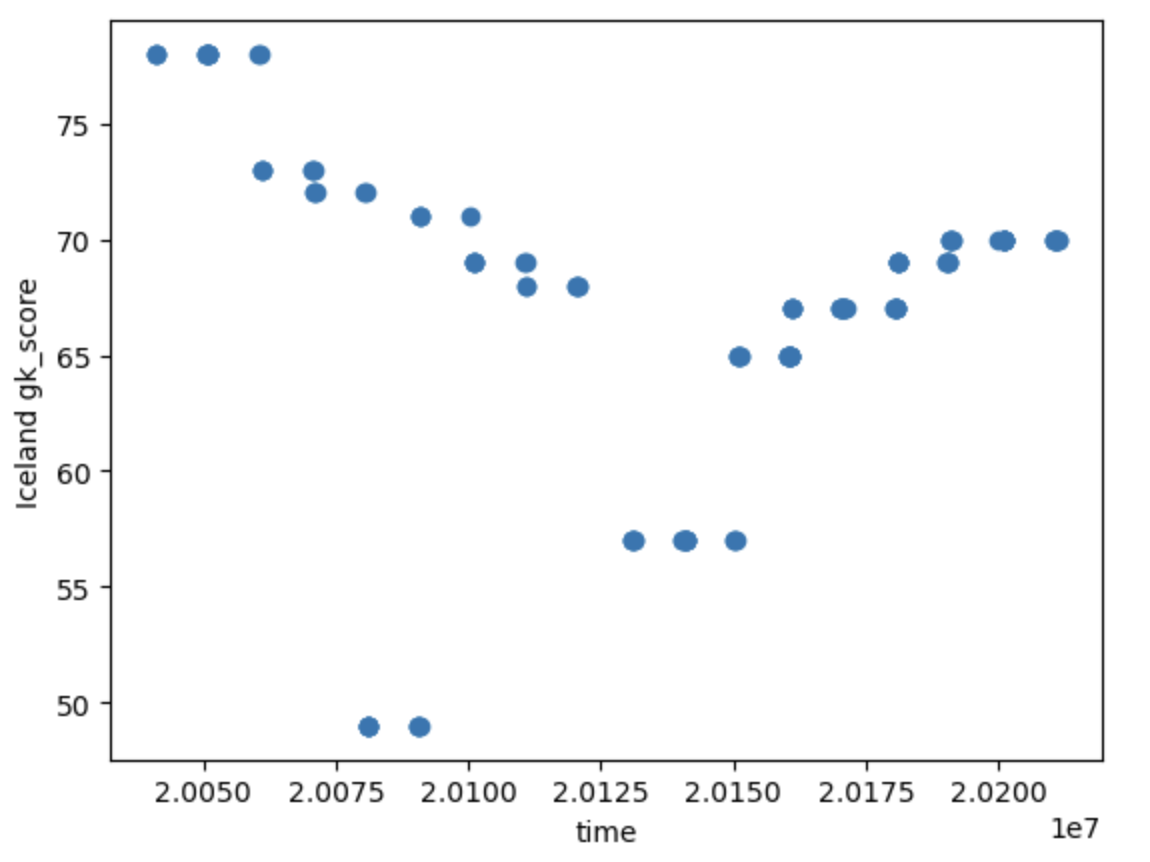
\includegraphics[scale=.3]{ice_gk_values.png}
    \caption{Examples to demonstrate randomness of plots}
    \label{fig:posscores}
\end{figure}
On the other hand, to predict TYPE2 missings, we attempted two different methods: 1.Regression with FIFA Rank, 2. Interpolation.

\textbf{Regression With FIFA Rank}\vspace{0.05cm}

An attempt to predict the missing values was to run a linear regression on the graphs according to Figure 1. After a thorough examination of the available options, it was determined that the linear regression method would be the most appropriate approach for the analysis, despite the observed increase in error as the FIFA rank increased. This decision was based on the consideration that the sample size significantly decreases as the FIFA rank increases, and the linear regression method was deemed to be the most suitable method of analysis under such circumstances. The linear regression model was constructed given the FIFA rank and position score information.

\textbf{interpolate()}\vspace{0.05cm}

\textit{pandas.Series.interpolate()} \cite{interpolate} is a library method than can interpolate values in a dataset in which `NaN' values are present. By creating, for each feature, a \textit{pandas.Series} containing every instance of that feature (whether it is missing or not) along with the rank of the country for which the value belongs, we can interpolate the missing values. This allows us to, for example, create an artificial value for Zambia's average \textit{defense\_score}. This method of interpolation can be done either linearly or polynomially - looking at the data representation in Figure 1, linear interpolation was chosen. Below is an example of how linear interpolation works:

\tiny{
\begin{python}
    >>> s = pd.Series([0, 1, np.nan, 3])
    >>> s
    0    0.0
    1    1.0
    2    NaN
    3    3.0
    dtype: float64
    >>> s.interpolate()
    0    0.0
    1    1.0
    2    2.0
    3    3.0
    dtype: float64
\end{python}
}
\small

\textbf{Gaussian Distribution}\vspace{0.05cm}

In addition to these approaches, we also attempted to predict TYPE1 and TYPE2 missings simultaneously. We modelled a country's position scores as a Gaussian random variable. To do this, we first gathered all records of the country's missing position score from the \textit{match\_history.csv} file. Then, the mean and variance could be calculated using the NumPy functions \textit{mean()} and \textit{var()}. An important decision we made was to use a truncated Gaussian distribution. Extrapolating above or below the observed best and worst performances for a team could potentially bias our data, especially since the Gaussian distribution is symmetrical.
Computationally, this method proved near equivalent to calculating averages. This is because the extra work of calculating the variance and then sampling from the truncated Gaussian distribution was small compared to iterating through the dataset to gather the relevant data.

\begin{figure}[H]
        \centering
        \begin{subfigure}[b]{0.45\textwidth}
            \centering
            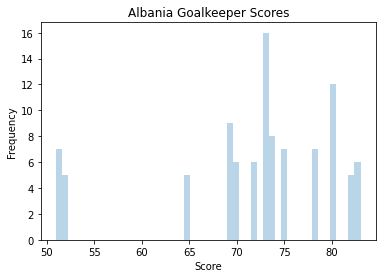
\includegraphics[scale=.4]{albania_scores.png}
            \caption{Real Scores}
        \end{subfigure}
        \hspace{0.5em}%
        \begin{subfigure}[b]{0.45\textwidth}
            \centering
            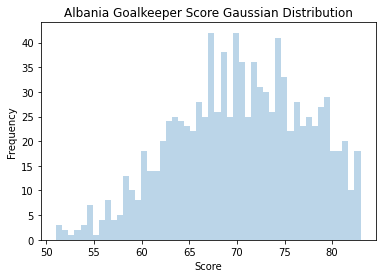
\includegraphics[scale=.4]{albania_gaussian.png}
            \caption{Simulated Scores}
        \end{subfigure}
        \caption{Comparison of real and simulated results for Albania's \textit{goalkeeper\_score}, presented as histograms}
        \label{fig:histograms}
\end{figure}
Using the truncated Gaussian distribution replicated the naturally occurring variance in the data well and without extrapolation. However, this method fell short when dealing with instances of features being completely absent for a country, as mentioned in \hyperref[sec:miss sec]{Section 2.2}.

\section{Methodology}
With the cleaned data prepared, our team decided to begin by experimenting with various approaches and analysing their predictions before committing to a single model.

As the predictions for the football matches can be split into 3 classes (win = 1, draw = 0, loss = -1), our team's intuition was to test simple methods that support multi-class classification. We implemented several baseline models using methods covered in class, including Logistic Regression, Naïve Bayes and Gaussian Naïve Bayes [yet to implement]. The idea was to let the performances of these models without any significant adjustments guide us towards the most suitable approach.

We tested a few novel methods after obtaining results from the baseline models. The team applied k-Nearest Neighbour (KNN) clustering and a Support Vector Machine (SVM) model to fit the data. We also implemented two neural networks, including a  Multi-layer perceptron (MLP) with scikit-learn and a 5-layer Convolutional Neural Network (CNN) with Keras to produce mock models to test.
\label{sec:others}

\subsection{Background and Literature Review}

%research with links to the currently used methods and approaches
The usage of machine learning to predict sports results is a growing area that requires high predictive accuracy. This is especially important now because of the large amount of money involved in sports betting as well as because sports managers could use it for strategy modelling. Football is the most popular sport in the world and accounts for the largest sports betting industry market share of more than 23.0\% and it is expected to increase in the future. \cite{footballstats} 
In 2021, the global sports betting market had a value of \$74.2 Billion with a prediction to grow to \$129.3 Billion by 2028. \cite{footballstats2} 
Therefore, creating a machine learning model that can accurately predict international FIFA results would be of a high impact
 
The first approaches of statistical modelling used for the prediction of football match scores were published in 1953 by Moroney \cite{moroney} 
and in 1971 by Reep,\cite{reep} 
where they used historical match results in Poisson and negative binomial distributions. Then, in 1974 Hill \cite{hill}
proved that match results can indeed be predicted and are not based on chance only. One of the earliest publications that used modern ML algorithms was published in 2005 by Goddard which used an ordered regression model.\cite{goddard}
 Later on, a study published in 2011 by Hucaljuk and Rakipovic compared several ML techniques and algorithms for football scores prediction, which included Artificial Neural Networks, Random Forest, KNN, LogiBoost, Bayesian Networks, and Naïve Bayes, and concluded that the best accuracy was achieved using ANN.\cite{hucaljuk} Additionally, considering feature reduction techniques In 2015, Tax concluded that PCA dimensionality reduction combined with a Multilayer Perception classifier and Naïve Bayes achieved the highest accuracy. \cite{dutch}
In 2016, Tavacol used feature extraction and aggregation methods to decrease the amount of features for the training of his model. \cite{tavakol}

Currently, since results can be classified into lose, win or draw classes, it is normally considered a classification problem. However, there are publications where it is considered a numeric prediction problem and the winning margin is predicted as a numeric value, but this method is rare. Most of the published papers include feature selection and feature extraction before the use of the machine-learning algorithm. In addition, as an evaluation method, researchers mostly use data segmentation  with chronological distribution and the k-cross evaluation method.\cite{anotherone} 
A standard approach would typically be based on historical match results, indicators of players' performance and information on the opposition. \cite{bunkerthabtah} The most common supervised ML algorithms used for sports analysts are decision trees, linear regression, naïve Bayes and neural networks, as well as unsupervised ML algorithms like k-means.

\begin{figure}[H]
    \centering
    %\resizebox{0.7\columnwidth}{!}{
    \begin{tabular}{ |p{4cm}||p{4cm}|p{3cm}|p{4cm}| }

\hline
Authors & Year & Accuracy & Method \\
\hline
Igiri and Nwachukwu & 	2014 & 	93\% & 	LR \\ 
Mustafa et al & 	2017 & 	87.9\% & 	SVM \\ 
Ping-Feng et al. & 	2017 & 	85.25\% & 	SVM \\ 
Horvat et al & 	2018 & 	83.96\% & 	KNN \\ 
Ganduly and Frank & 	2018 & 	82\% & 	Neural network \\ 
Purucker & 	1996 & 	78.6\% & 	Neural network \\ 
Zimmermannet al & 	2013 & 	74.46\% & 	MLP \\ 
Loeffelholzet al & 	2009 & 	74.33\% & 	Neural network \\ 
Zdravevski andKulako & 	2010 & 	72.8\% & 	LR \\ 
Zaveri at al. & 	2018 & 	71.63\% & 	LR \\ 
Kravanja & 	2013 & 	70.01\% & 	SVM \\ 
Cao & 	2012 & 	69.67\% & 	LR \\ 
Prasetio andHarlili  & 	2016 & 	69.5\% & 	LR \\ 
Hubácˇek et al & 	2019 & 	68.83\% & 	Neural network \\ 
Hamadani & 	2006 & 	67.08\% & 	LR \\ 
Soto Valero & 	2016 & 	58.92\% & 	SVM \\ 
Buursma & 	2011 & 	57\% & 	LR \\ 

\hline
\end{tabular}
%}
    \caption{Published papers with their best predicted accuracy \cite{horvat}}
    \label{fig:table}
\end{figure}

\subsection{Modelling Approaches}
%brief overview of the approaches we took (further discussed in the next section)
Most of the following approaches are commonly used for performing linear or nonlinear classification, regression and the detection of outliers. Therefore to predict football match outcomes that has 3 classes (1 for win, 0 for draw and -1 for loss), we need to adopt a One-vs-Rest (OVR) strategy to facilitate multinomial classification. This approach projects the input data to a higher-dimensional space that allows mutual linear separation between every two classes \cite{baeldung}. The projected data can then be classified after training n binary linear classifiers for each class.

\subsubsection{Support Vector Machines (SVM)}
SVM is a supervised Machine Learning algorithm that is commonly used for performing linear and nonlinear classification, regression and the detection of outliers. The objective of SVMs is to realize a hyperplane that maximises the separation between groups of data points in an n-dimensional feature space \cite{baeldung}. The data points with the minimum distance to the hyperplane are the Support Vectors.

Our SVM approach was combined with the OVR strategy to predict match outcomes. There was a weak sensitivity towards matches resulting in a draw.

\subsubsection{Logistic Regression}
Multinomial logistic regression is considered as a reasonable choice for fitting the data since it can predict more than two classes of discrete outcomes. We implemented this in sklearn by setting the Logistic Regression class parameters explicitly: multi\_class='multinomial'.

This approach gave us the advantage of handling highly interpretable coefficients to compare the features and outcome values. This methodology has the advantage of flexibility over simple logistic regression which enables us to make no assumptions about the distributions in the feature space. Furthermore, the calculations with the logistic regression are performed through the arithmetic problem with probability. This approach enabled us to visualise the accuracy of the prediction as a numerical value, especially with the low-dimensional dataset.

\subsubsection{k-Nearest Neighbours (KNN)}
K-Nearest Neighbours clustering can be used for both classification and regression. For predicting football match outcomes, KNN can classify the match results of unseen matches using labelled observations by finding the K-closest data points surrounding the unseen data point.

Assuming that examples of the same match outcome have similar features, that is, the proximity of each data point is tiny given they come from the same match outcome, then KNN is a promising approach since we can form 3 clusters for each possible match outcome (win, draw, loss).

The accuracy of our KNN implementation varies with the value of K (number of neighbours to consider). A small value of K will produce unstable decision boundaries for classifying an unseen data point. In our implementation, we used K=40 to train our KNN model.

\subsubsection{Multilayer perceptron (MLPNN)}
A multilayer perceptron can learn a non-linear function approximator for classification. Contrary to logistic regression, it can have multiple hidden (non-linear) layers with activation functions. This enables the potential to learn non-linear models that may fit the data better.

Therefore, it is widely known for solving problems with supervised learning such as the backpropagation technique each of the data samples has labelling to its belongings. We have utilised this technique to train the data set by learning the patterns with based on the error calculation between the prediction and the actual value.

This uses a similar transfer function as logistic regression but it uses the step function instead of the logistic function. This approach could handle a large amount of data sets with similar accuracy which is achieved with smaller data sets.

\section{Model Training and Evaluation}
\subsection{Data Pre-processing and Partitioning}

The dataset was split into training and testing data using a 80:20 split. It initially consists of 25 feature columns and 5641 examples (tuples). The match\_result data [Win, Lose, Draw] was transformend into [1,0,-1], There are 1525 rows ith missing data in the dataset, which were dealt with as in \hyperref[sec:exploration]{Section 2} . Some columns that were not used were removed as they do not serve purpose in this work.

\subsection{Data Resampling}
We tried to resample the data to gather more information for each sample. This approach has proceeded by drawing the samples from the different training sets, enabling us to inspect how data yields different outputs for the different training sets.
The dataset is imperfect with missing values of the team mean defence, offence and goalkeeper scores, therefore we have tried to resample the data by predicting with regularisation to yield better accuracy for the results.

\begin{enumerate}
    \item Regularisation could prevent overfitting due to the low bias and high variance on the prediction of the dataset.
    \item No sampling
\end{enumerate}

Our team trained the interpolated dataset on the models proposed in Section 3.2. We tested these fitted models in a separate test set and achieved an accuracy of more than 90\% across all models.

We considered this outcome as a potential sign of overfitting. Therefore, we spent some time analysing the interpolated dataset for errors. After some analysis, we found that the interpolated dataset contained both the \textit{home\_team\_score} and \textit{away\_team\_score} features. Since these two features can directly determine the outcome of a match, it is considered as a dominant feature pair amongst the whole dataset, which caused our models to become strongly biased towards these features, explaining why our models have overfitted.

Removing the \textit{home\_team\_score} or \textit{away\_team\_score} feature columns proved to boost the accuracy of our models by around 10\%.


\subsection{Feature Engineering}
The goal of feature engineering is to eliminate redundant data which speeds up the data transformation to yield better accuracy for the predictions. This has been approached by handling the missing data and normalising the data for further exploratory analysis and investigation.

We performed some experiments to discount the prediction for the missing data by comparing the outputs for accuracy with various methods of each prediction model. The methods are:
\begin{enumerate}
    \item Outlier handling improved the data prediction especially by replacing the NaN values with the value from the imputation 
    \item Imputation helped to handle the missing values in the data set. The missing values can affect the performance of the machine learning models. We tried to fill in the missing data by predicting based on the data remainder such as the Fifa rank for each country.
\end{enumerate}

We implemented four new features for our dataset, computed using pre-existing values: \textit{home\_team\_total\_average}, \textit{away\_team\_total\_average}, \textit{goal\_difference}, and \textit{home\_team\_rank\_difference}. These four new features represent, the average of the four aforementioned score feature values, for both the home and away teams, the absolute value of the goal difference in the game, and the difference between the home and away teams' FIFA ranks, respectively. 

The addition of these features improved model accuracy across the board, by around 7\%. It must however be noted that, with similar reasoning to the removal of the \textit{home\_team\_score} and \textit{away\_team\_score}, the \textit{goal\_difference} feature could in some circumstances be used, singularly, by the model to predict the outcome of a match, disregarding other features. This is due to the fact that no matter how many goals were scored, or the performance of either team's players, if the goal difference is zero, the match has to have been a draw. It follows that our models may slightly over-fit data with a bias towards draws - which in the original dataset accounts for around one quarter of the total games.

\subsection{Scoring}
We computed 4 metrics to choose between the interpolated and linear regression datasets: accuracy, precision, recall and F-score. The F-score in particular, is a measure of a test's accuracy, which is calculated from the precision and recall of the test. The highest possible F-score is 1.0 indicating perfect precision and recall, while the lowest value is 0.0 if either precision or recall is 0.

The match outcomes in the original, non-transformed dataset are slightly \textit{unbalanced} - 2605 wins, 1387 draws and 1649 loses. Hence, the common approach to scoring a model using accuracy is not as reflected in this project. We decided to use the F-score as our scoring method to determine which dataset we will use for our models (refer to \ref{fig:tableA} and \ref{fig:tableB} in Section 5.1).

\subsection{Optimisation and Model Selection}
The goal of the optimisation is to adjust the data set by prioritising the criteria or restricting the data set with constraints. This enabled us to design the data set by eliminating redundant data for better performance. The goal of the model selection is to decide the best model among the candidates which performs the best. After we choose which dataset to use as in Section 4.5, we train our models on the feature-engineered version of the dataset. Finally, we evaluate each of our models by ranking their F-scores and choosing the model with the highest F-score for final testing (refer to \ref{fig:tableC} in Section 5.1).

\subsection{Further Improvements}
Potential improvements include performing further optimisation to reduce the time cost for the calculation of the missing data which we are handling, which would improve the visualisation of the data. In addition, performing various modelling approaches that would give us more options to choose the better accuracy for the data prediction.
Moreover, more types of data could be included in the dataset so that the prediction can be made more precisely. In order to improve further accuracy, we could verify each step of the data modelling before moving on to the next stage. This approach could prevent the data is considered multiple times which can be regarded as redundant data.

\section{Results and Final Predictions on Test Set}
Now we will present the results of our models, showing the impact various methods had on their accuracy.
So as to not discount an approach too early, we tested every model at every step of our methodology and compared the results below.
Our ultimate choice in model and methods applied was heavily, but not entirely, influenced by accuracy.

\subsection{Initial Performance}
We began by running each model type on the interpolated and linear regression reconstructed datasets. These results served as a baseline which we would use to compare against going forwards.

\begin{figure}[H]
    \centering
 %   \resizebox{0.7\columnwidth}{!}{
    \begin{tabular}{ |p{3cm}||p{3cm}|p{3cm}|p{3cm}|p{3cm}| }
\hline
Scoring method & LR & SVM & KNN & MLP \\
\hline
 Accuracy & 0.5252 & 0.5137 & 0.5049 & 0.5279\\
 F-score & 0.4067 & 0.3598 & 0.4177 & 0.3985\\
 Precision & 0.5594 & 0.5169 & 0.4518 & 0.5839\\
 Recall & 0.4600 & 0.4093 & 0.4546 & 0.4516\\
\hline
\end{tabular}
%}
    \caption{Base Model Results on Interpolated Dataset without feature engineering}
    \label{fig:tableA}
\end{figure}
\begin{figure}[H]
    \centering
 %   \resizebox{0.7\columnwidth}{!}{
    \begin{tabular}{ |p{3cm}||p{3cm}|p{3cm}|p{3cm}|p{3cm}| }
 \hline
 Scoring method & LR & SVM & KNN & MLP\\
 \hline
 Accuracy & 0.5474 & 0.5102 & 0.5323 & 0.5447\\
 F-score & 0.3850 & 0.3614 & 0.3905 & 0.4151\\
 Precision & 0.3352 & 0.4466 & 0.4213 & 0.4845\\
 Recall & 0.4532 & 0.4209 & 0.4395 & 0.4514\\
\hline
\end{tabular}
%}

    \caption{Base Model Results on Linear Regression Dataset without feature engineering}
    \label{fig:tableB}
\end{figure}
% Figure [x], standard model accuracies on base dataset

% As displayed in figure [x], performance across all models was poor at around 50\%.
% (might need to run this again without any transformation of the dataset, just as it is given to us)

\subsection{Model Optimisations and Regularisation}
From Section 5.1, we decide to use the interpolated reconstructed dataset. We then apply feature engineering to this dataset and evaluate each model using the F-scores. The following table summarises the metrics for each model under the interpolated dataset:
\begin{figure}[H]
    \centering
 %   \resizebox{0.7\columnwidth}{!}{
    \begin{tabular}{ |p{3cm}||p{3cm}|p{3cm}|p{3cm}|p{3cm}| }
 \hline
 Scoring method & LR & SVM & KNN & MLP\\
 \hline
 Accuracy & 0.7874 & 0.6997 & 0.5279 & 0.7724\\
 F-score & 0.7881 & 0.6756 & 0.4089 & 0.7514\\
 Precision & 0.7917 & 0.7458 & 0.4485 & 0.7935\\
 Recall & 0.7902 & 0.6632 & 0.4497 & 0.7561\\
\hline
\end{tabular}
%}
    \caption{Base Model Results on Interpolated Dataset with feature engineering}
    \label{fig:tableC}
\end{figure}

Our most successful model was Logistic Regression - which by default performs some kind of $\ell_2$ regularisation. Upon turning off this default setting, we saw no remarkable difference in performance which suggests that the data had no features of low bias and high variance - so we chose to keep the default regularisation. It achieved the highest F-score out of the four models with a score of 0.7881. 

\begin{figure}[H]
    \centering
    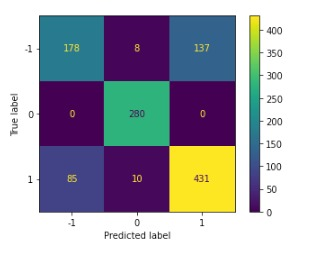
\includegraphics[scale=.5]{lr_cm_interpolated.jpeg}
    \label{fig:my_label}
    \caption{LR Confusion Matrix of the Interpolated Dataset with feature engineering}
\end{figure}

% \subsubsection{Class Weighting}

% \subsection{Dataset Optimisations}
% After failing to achieve any significant improvements through modifying the models alone, we quickly turned our attention to the data.
% The most glaring issue which stood out were the missing values present in the dataset.
% \subsection{Completing Data Using Mean}
% \subsubsection{Deleting Incomplete Rows}
% \subsubsection{Predicting Missing Data}
% \subsubsection{Creating New Features}
% (this could be the home advantage feature)
% \subsubsection{Transforming Features}
% (we turned win loss draw into numbers)
% (could also scale points, or create goal and rank difference features?)

% \section{\colorbox{yellow}{Final Predictions on Test Set}}
% We trained our logistic regression model on the interpolated dataset with feature engineering and achieved a predictive accuracy of xx.xx\%.
% [inset tables and graphs]




% (missclassification? overfitting? any patterns? train-test split effect? effect of skewed data?)


\section{Conclusion}
In conclusion, to prepare the data before inputting it into the model, various methods for replacing the missing data were tested, with replacing the missing data with country averages and values interpolated using FIFA rank being the most successful.
%Other methods of missing data treatment included the removal of rows, replacing them with a constant and replacing them with the overall dataset averages.
Testing of different, feature engineering and data sampling methods was conducted for four machine learning models: SVM, LR, KNN and MLP.
Overall, the best performing model was Logistic Regression using averages/interpolation reconstructed data with new features, with the predictive accuracy of 80.16\%. This means that there is a high chance for a correct match prediction, which would be profitable when used in sports betting. These results are lower than the accuracy from the literature which can be explained by the use of different input data, different models and different data splits.
%To improve the predictive accuracy of the model, improvements to the model can include further optimisation of the missing data as well as performing more modelling approaches.

\bibliographystyle{unsrt}  
\bibliography{references}  %%% Remove comment to use the external .bib file (using bibtex).
%%% and comment out the ``thebibliography'' section.
%\tiny

%%% Comment out this section when you \bibliography{references} is enabled.
\begin{thebibliography}{1}

\bibitem{missing_data}
    Sunil Ray
    \newblock \textit{``A Comprehensive Guide to Data Exploration''}
    \url{https://www.analyticsvidhya.com/blog/2016/01/guide-data-exploration/}
% References for Section 3 (Methodology)
\bibitem{horvat}
Horvat, T. and Job, J. (2020) \textit{``The use of machine learning in sport outcome prediction: A Review,}'' WIREs Data Mining and Knowledge Discovery, 10(5). Available at: \url{https://doi.org/10.1002/widm.1380}. 

\bibitem{footballstats} 
Global sports betting market size; growth report, 2030 (2022) Global Sports Betting Market SIze; Growth Report, 2030. Available at: \url{https://www.grandviewresearch.com/industry-analysis/sports-betting-market-report}

\bibitem{footballstats2}
Vantage Market Research {\em Vantage Market Research (2022) Sports betting market size}. GlobeNewswire News Room. Available at: \url{https://www.globenewswire.com/en/news-release/2022/11/16/2556991/0/en/Sports-Betting-Market-Size-Share-to-Surpass-USD-129-3-Billion-by-2028-Vantage-Market-Research.html}

\bibitem{moroney}
Moser, C.A. and Moroney, M.J. (1953) {\em “Facts from figures.,”} Economica, 20(77), p. 91. Available at: \url{https://doi.org/10.2307/2551006.}

\bibitem{reep}
Reep, C., Pollard, R. and Benjamin, B. (1971) {\em“Skill and chance in ball games,”} Journal of the Royal Statistical Society. Series A (General), 134(4), p. 623. Available at: \url{https://doi.org/10.2307/2343657.} 

\bibitem{hill}
Hill, I.D. (1974) {\em“Association football and Statistical Inference,”} Applied Statistics, 23(2), p. 203. Available at: \url{https://doi.org/10.2307/2347001}.

\bibitem{goddard}
Goddard, J. (2005) \textit{“Regression models for forecasting goals and match results in association football,”} International Journal of Forecasting, 21(2), pp. 331–340. Available at: \url{https://doi.org/10.1016/j.ijforecast.2004.08.002}. 

\bibitem{hucaljuk}
J. Hucaljuk and A. Rakipović, \textit{"Predicting football scores using machine learning techniques,"} 2011 Proceedings of the 34th International Convention MIPRO, Opatija, Croatia, 2011, pp. 1623-1627.

    
   \bibitem{dutch}
    Tax, N., Yme Joustra, 2015. \textit{Predicting The Dutch Football Competition Using Public Data: A Machine Learning Approach. } \url{https://doi.org/10.13140/RG.2.1.1383.4729}

\bibitem{tavakol} 
Tavakol, Maryam, Zafar, Hamid, Brefeld, Ulf. (2016). \textit{Feature Extraction and Aggregation for Predicting the EURO 2016.} Available at: \url{https://www.researchgate.net/publication/306393307_Feature_Extraction_and_Aggregation_for_Predicting_the_EURO_2016}


    \bibitem{anotherone}
    Horvat, T. and Job, J. (2020) 
    \newblock  {\em`“The use of machine learning in sport outcome prediction: A Review"}
    \newblock WIREs Data Mining and Knowledge Discovery, 10(5). Available at: \url{https://doi.org/10.1002/widm.1380}.


 \bibitem{bunkerthabtah}
    Bunker, R.P. and Thabtah, F. (2019).
    \newblock  {\em``A machine learning framework for sport result prediction''}
    \newblock In Applied Computing and Informatics, 15(1), pp. 27–33. Available at: \url{https://doi.org/10.1016/j.aci.2017.09.005}.

\bibitem{interpolate}
\textit{pandas.Series.interpolate}. Available at: \url{https://pandas.pydata.org/docs/reference/api/pandas.DataFrame.interpolate.html}


\bibitem{baeldung}
    Baeldung
    \textit{Multiclass Classification Using Support Vector Machines},
    2022,
    \url{https://www.baeldung.com/cs/svm-multiclass-classification}




% \bibitem{kour2014fast}
% George Kour and Raid Saabne.
% \newblock Fast classification of handwritten on-line arabic characters.
% \newblock In {\em Soft Computing and Pattern Recognition (SoCPaR), 2014 6th
%   International Conference of}, pages 312--318. IEEE, 2014.

% \bibitem{hadash2018estimate}
% Guy Hadash, Einat Kermany, Boaz Carmeli, Ofer Lavi, George Kour, and Alon
%   Jacovi.
% \newblock Estimate and replace: A novel approach to integrating deep neural
%   networks with existing applications.
% \newblock {\em arXiv preprint arXiv:1804.09028}, 2018.

\end{thebibliography}


\end{document}

%\lipsum[8] \cite{kour2014real,kour2014fast} and see \cite{hadash2018estimate}.

%The documentation for \verb+natbib+ may be found at
%\begin{center}
  %\url{http://mirrors.ctan.org/macros/latex/contrib/natbib/natnotes.pdf}
%\end{center}
%Of note is the command \verb+\citet+, which produces citations
%appropriate for use in inline text.  For example,
%\begin{verbatim}
   %\citet{hasselmo} %investigated\dots
%\end{verbatim}
%produces
%\begin{quote}
%  Hasselmo, et al.\ (1995) investigated\dots
%\end{quote}

%\begin{center}
  %\url{https://www.ctan.org/pkg/booktabs}
%\end{center}
%\lipsum[5]
%\begin{equation}
%\xi _{ij}(t)=P(x_{t}=i,x_{t+1}=j|y,v,w;\theta)= {\frac {\alpha _{i}(t)a^{w_t}_{ij}\beta _{j}(t+1)b^{v_{t+1}}_{j}(y_{t+1})}{\sum _{i=1}^{N} \sum _{j=1}^{N} \alpha _{i}(t)a^{w_t}_{ij}\beta _{j}(t+1)b^{v_{t+1}}_{j}(y_{t+1})}}
%\end{equation}
%\lipsum[12]
%See awesome %Table~\ref{tab:table}.

%\begin{table}
% \caption{Sample table title}
%  \centering
%  \begin{tabular}{lll}
%    \toprule
%    \multicolumn{2}{c}{Part}                   \\
%    \cmidrule(r){1-2}
%    Name     & Description     & Size ($\mu$m) \\
 %   \midrule
 %   Dendrite & Input terminal  & $\sim$100     \\
  %  Axon     & Output terminal & $\sim$10      \\
   % Soma     & Cell body       & up to $10^6$  \\
 %   \bottomrule
 % \end{tabular}
  %\label{tab:table}
%\end{table}
%\begin{itemize}
%\item Lorem ipsum dolor sit amet
%\item consectetur adipiscing elit. 
%\item Aliquam dignissim blandit est, in dictum tortor gravida eget. In ac rutrum magna.
%\end{itemize}

%\lipsum[10] 
%See Figure \ref{fig:fig1}. Here is how you add footnotes. \footnote{Sample of the first footnote.}
%\lipsum[11] 

%\begin{figure}
 % \centering
  %\fbox{\rule[-.5cm]{4cm}{4cm} \rule[-.5cm]{4cm}{0cm}}
  %\caption{Sample figure caption.}
  %\label{fig:fig1}
%\end{figure}
